\documentclass[a4paper,11pt]{texMemo}
\usepackage[english]{babel}
\usepackage{graphicx}
\usepackage{float}
\memoto{Prof. Dave Hale, Prof. T.K. Young}
\memofrom{Colton Kohnke}
\memodate{October 7, 2013}
\memosubject{GPGN438 Project Progress Report}

\begin{document}
\maketitle

This memo is to report on the progress that has been completed for the senior design project for GPGN438 titled ``Exploratory seismic data analysis in the field.'' \\

To date, I have been utilizing the Mines JAVA Toolkit (Mines JTK) to refamiliarize myself with JAVA plotting and interactive display functions. Specifically, the JTK has a demo java file called PolesAndZeroes.java that utilizes the JTK mosaic package to create an interactive display. Using this demo as a base, I was able to create a base plot that will function as a map view of the survey geometry and a second plot that will become a plot of the geophone signal (Figure 1). \\

\begin{figure}[H]
\centering
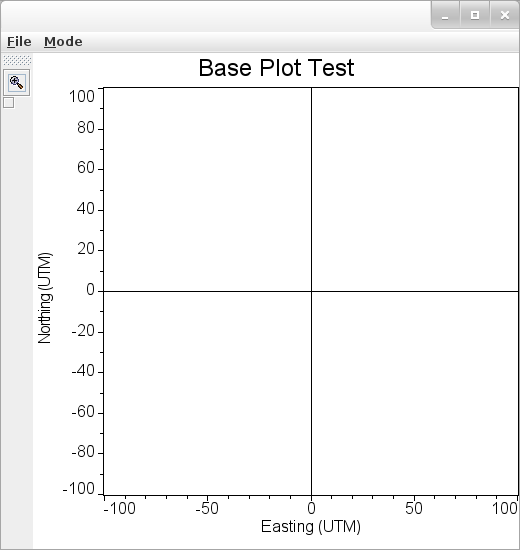
\includegraphics[scale=.3]{plot1.png} 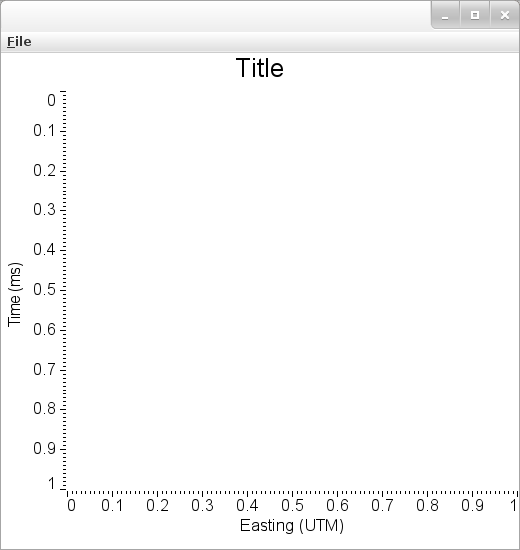
\includegraphics[scale=.3]{plot2.png}
\caption{Test base plot map image (left) and geophone response testing space (right). This figure is behind by 2 git commits.} 
\end{figure}

In order to test adding points to the base map, I created an add point method. This method is currently broken in the area where pixels are converted to and from real values. The method plots points, but not at the clicked location. I was anticipating an easy fix, however I think there are some hidden limitations to converting data types (double, int, float) to represent the large UTM values. I need to complete more thorough analysis of this situation before completion of this method can be completed for testing. \\

I have also added skeleton menu items (not depicted in Figure 1) to be implemented and tested in the future. These include:
\begin{enumerate}
\item Get GPS from Handheld
\item Get DEM Model from USGS
\item Import from segy
\item Export to CSV
\item Basic processing
\end{enumerate}

In addition, rough pseudo-code for interactively selecting and exploring the points on the base map have been written, but will not be implemented fully until the method that adds points to the base map is fixed. \\

Finally, an unforeseen consequence of the government shutdown is that the USGS DEM archives may be unavailable for an unknown amount of time. This may cause slowdowns in completing the method that obtains a DEM from the government site. I have not looked too deeply into this potential problem because it appears to be farther down the road and may not even be an issue. \\

In the upcoming month I plan to start implementing and testing different features, such as getting GPS from handheld, and exporting to CSV. I have also attached the expected project budget for the geophysics department. The "real world" budget will be completed at a later date. \\

\begin{figure}[ht]

\includegraphics[scale=.75]{Budget_Project.pdf}
\end{figure}

\end{document}
